\chapter{UML Diagrams}
Need to be added yet
\section{Domain Class Diagram}

\begin{figure}[h!t]
    \centering
    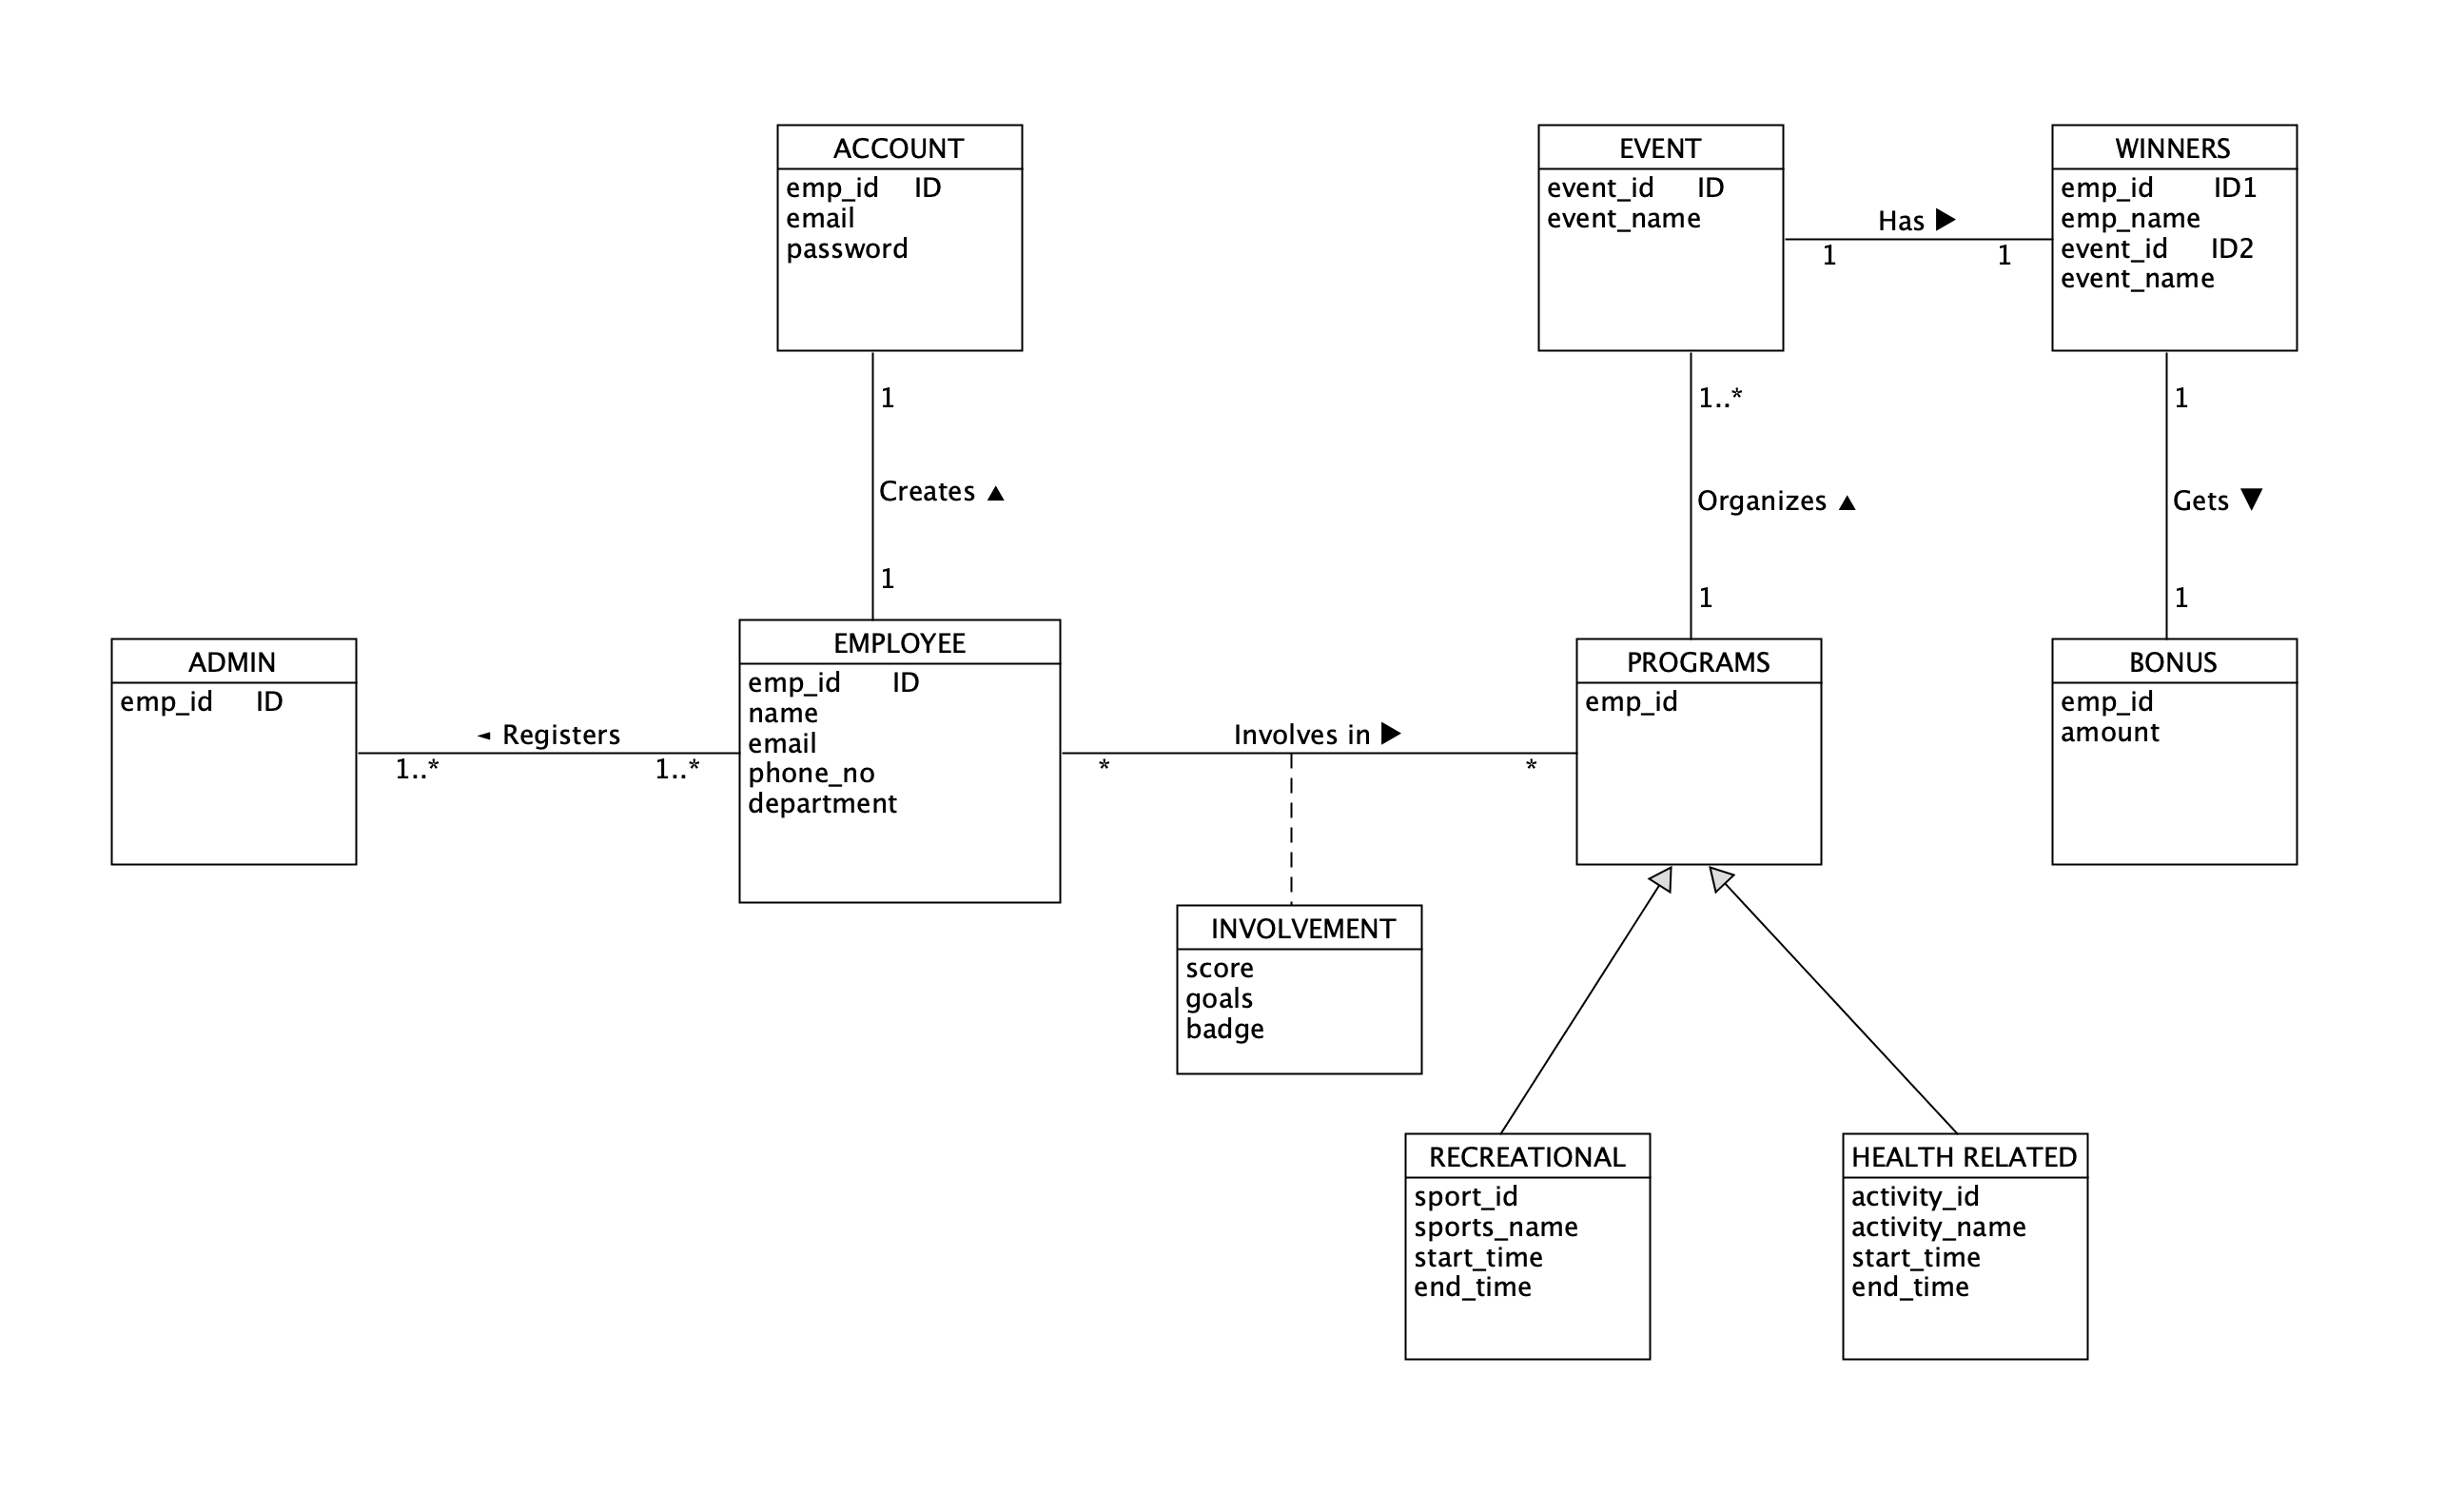
\includegraphics[width=\textwidth]{images/domainClass.png}
    \caption{Domain Class Diagram}
    \label{fig:domainClass}
\end{figure}

\section{Use Case Diagram}


\begin{table}[h!t]
\caption{The Registration Subsystem Use Cases}
{%
\newcommand{\mc}[2]{\multicolumn{#1}{#2}}
\begin{center}
\begin{tabular}{|c|c|}
\hline
\multicolumn{2}{|c|}{\textbf{RWIP Registration Subsystem}} \\ \cline{1-2}
\textbf{Use Cases} & \textbf{Users/Actors} \\
\hline
\rule{0pt}{24pt}  Create Account & Employee \\
\hline
\rule{0pt}{24pt}  Verify Account & Employee \\
\hline
\rule{0pt}{24pt}  Login to Account & Employee \\
\hline
\end{tabular}
\end{center}
}%
\label{tab:reg}
\end{table}

\begin{figure}[h!t]
    \centering
    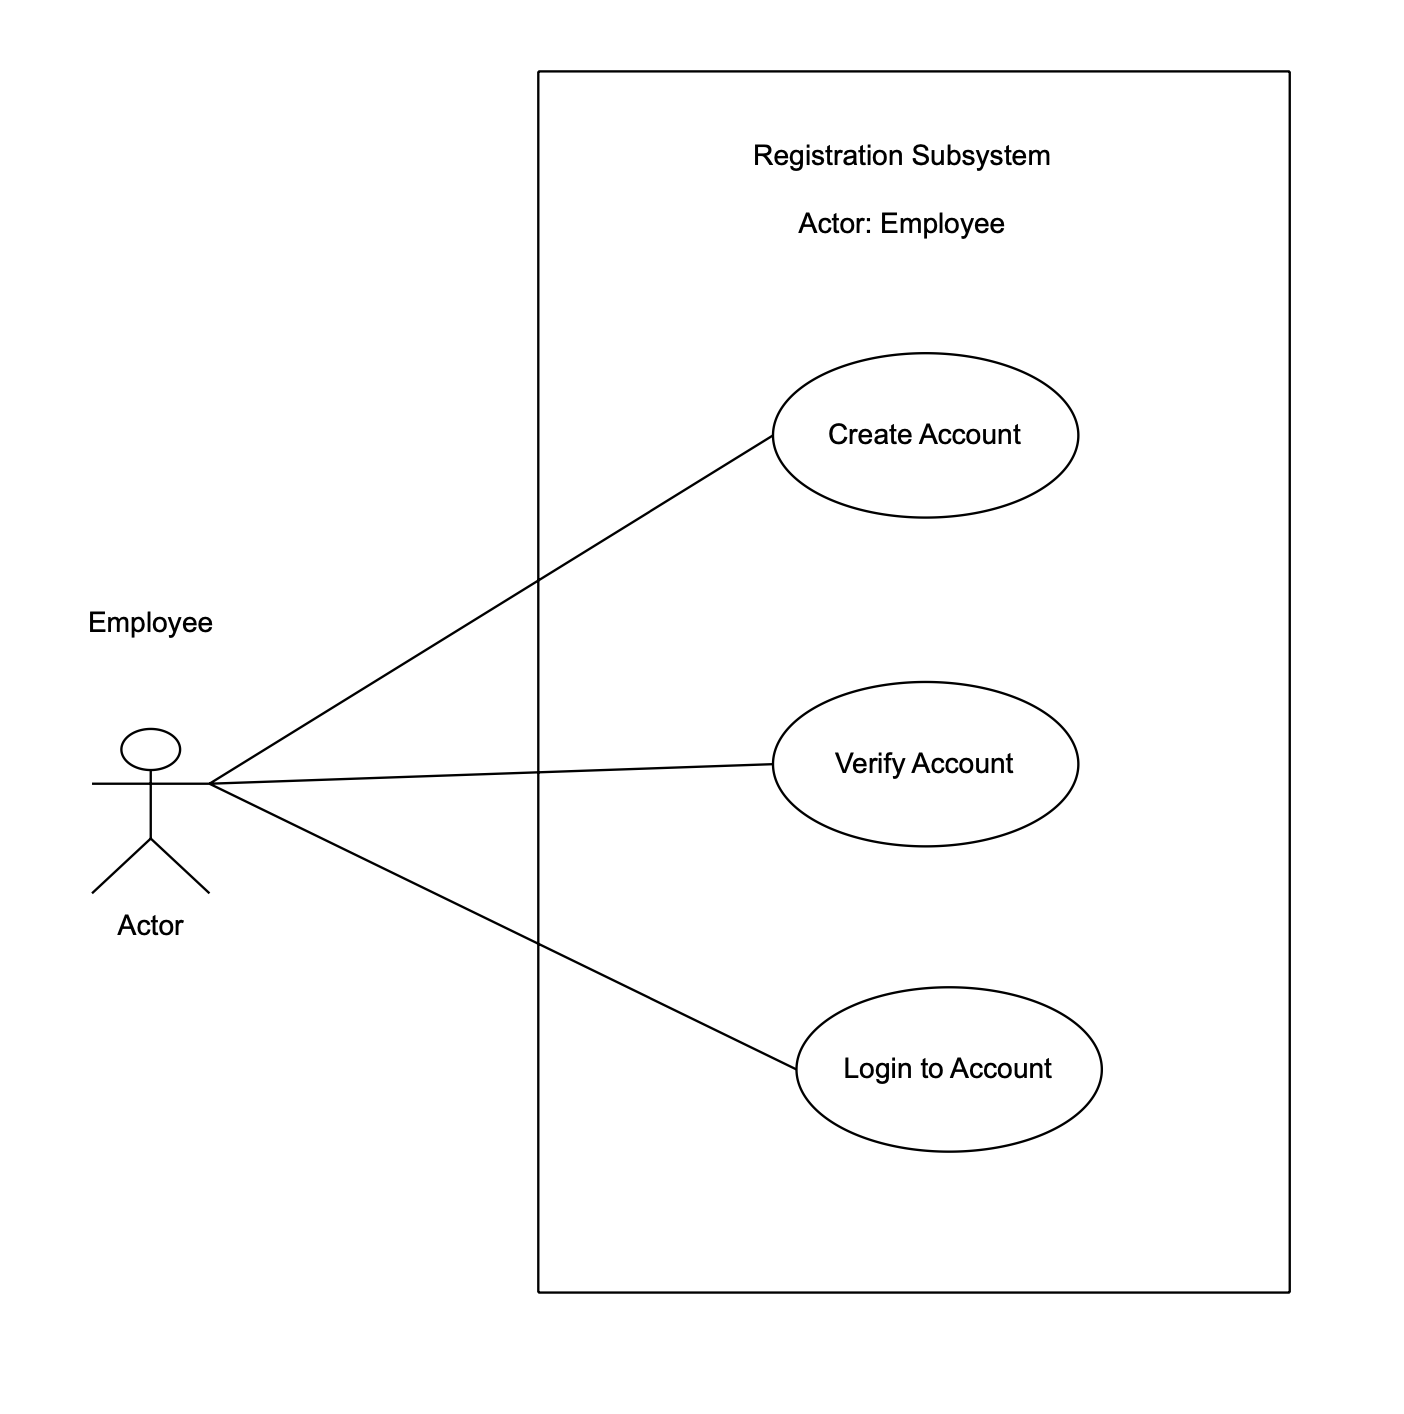
\includegraphics[width=\textwidth]{images/ucRegistration.png}
    \caption{Use case diagram for Registration subsystem}
    \label{fig:ucRegistration}
\end{figure}

\begin{table}[h!t]
\caption{The Program Subsystem Use Cases}
{%
\newcommand{\mc}[2]{\multicolumn{#1}{#2}}
\begin{center}
\begin{tabular}{|c|c|}
\hline
\multicolumn{2}{|c|}{\textbf{RWIP Program Subsystem}} \\ \cline{1-2}
\textbf{Use Cases} & \textbf{Users/Actors} \\
\hline
\rule{0pt}{24pt}  Login & Employee \\
\hline
\rule{0pt}{24pt}  Select Programs & Employee \\
\hline
\rule{0pt}{24pt}  Book/Enroll Programs & Employee \\
\hline
\rule{0pt}{24pt}  Participate in Programs & Employee \\
\hline
\rule{0pt}{24pt}  Update badges and rewards & Employee \\
\hline
\end{tabular}
\end{center}
}%
\label{tab:program}
\end{table}

\begin{figure}[h!t]
    \centering
    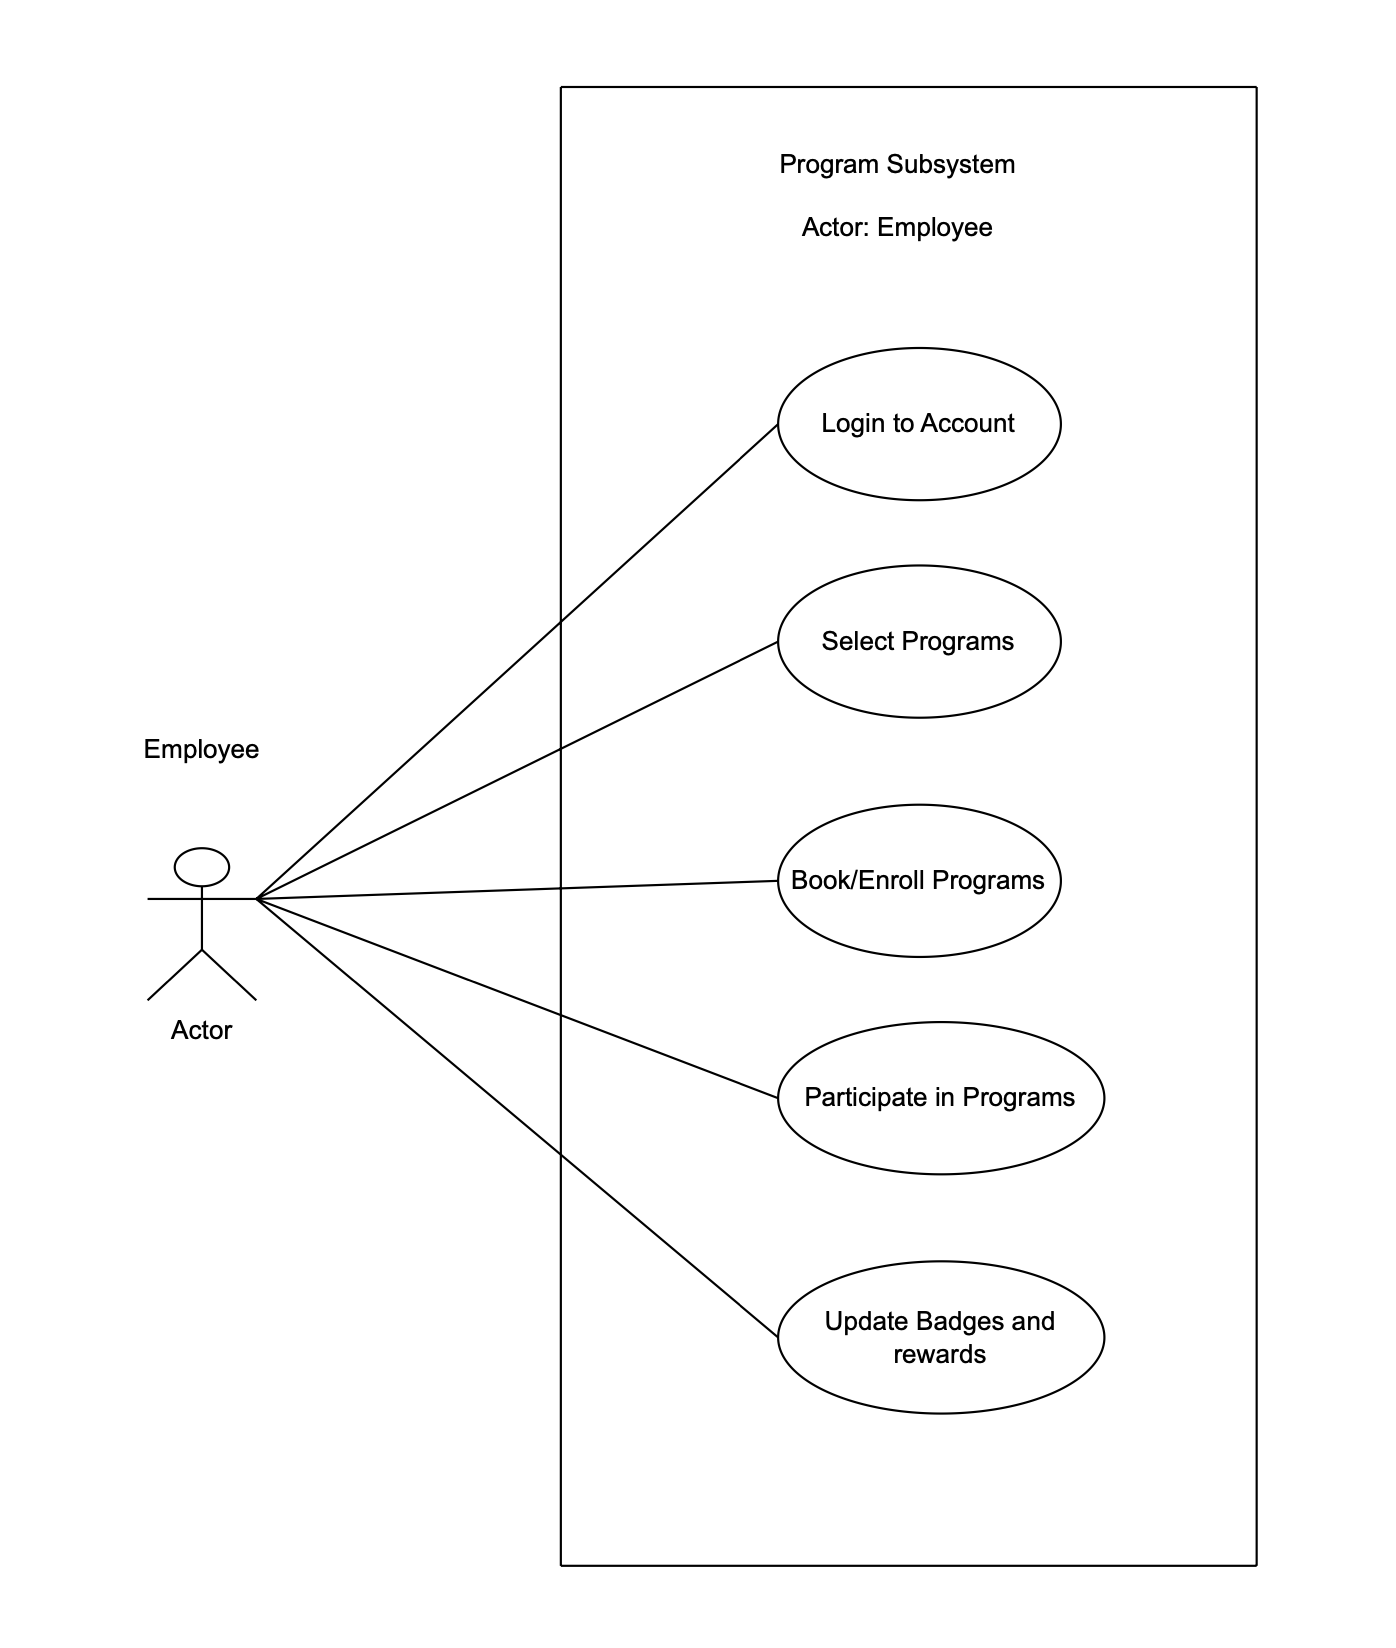
\includegraphics[width=\textwidth]{images/ucProgram.png}
    \caption{Use case diagram for Program subsystem}
    \label{fig:ucProgram}
\end{figure}


\begin{table}[h!t]
\caption{The Event Subsystem Use Cases}
{%
\newcommand{\mc}[2]{\multicolumn{#1}{#2}}
\begin{center}
\begin{tabular}{|c|c|}
\hline
\multicolumn{2}{|c|}{\textbf{RWIP Event Subsystem}} \\ \cline{1-2}
\textbf{Use Cases} & \textbf{Users/Actors} \\
\hline
\rule{0pt}{24pt}  Organise Events & HR/Admin \\
\hline
\rule{0pt}{24pt}  Notify Events & HR/Admin, Employee \\
\hline
\rule{0pt}{24pt}  Design Banner & HR/Admin \\
\hline
\rule{0pt}{24pt}  Participate in Events & Employee \\
\hline
\rule{0pt}{24pt}  Declare winners & HR/Admin, Employee \\
\hline
\end{tabular}
\end{center}
}%
\label{tab:event}
\end{table}

\begin{figure}[h!t]
    \centering
    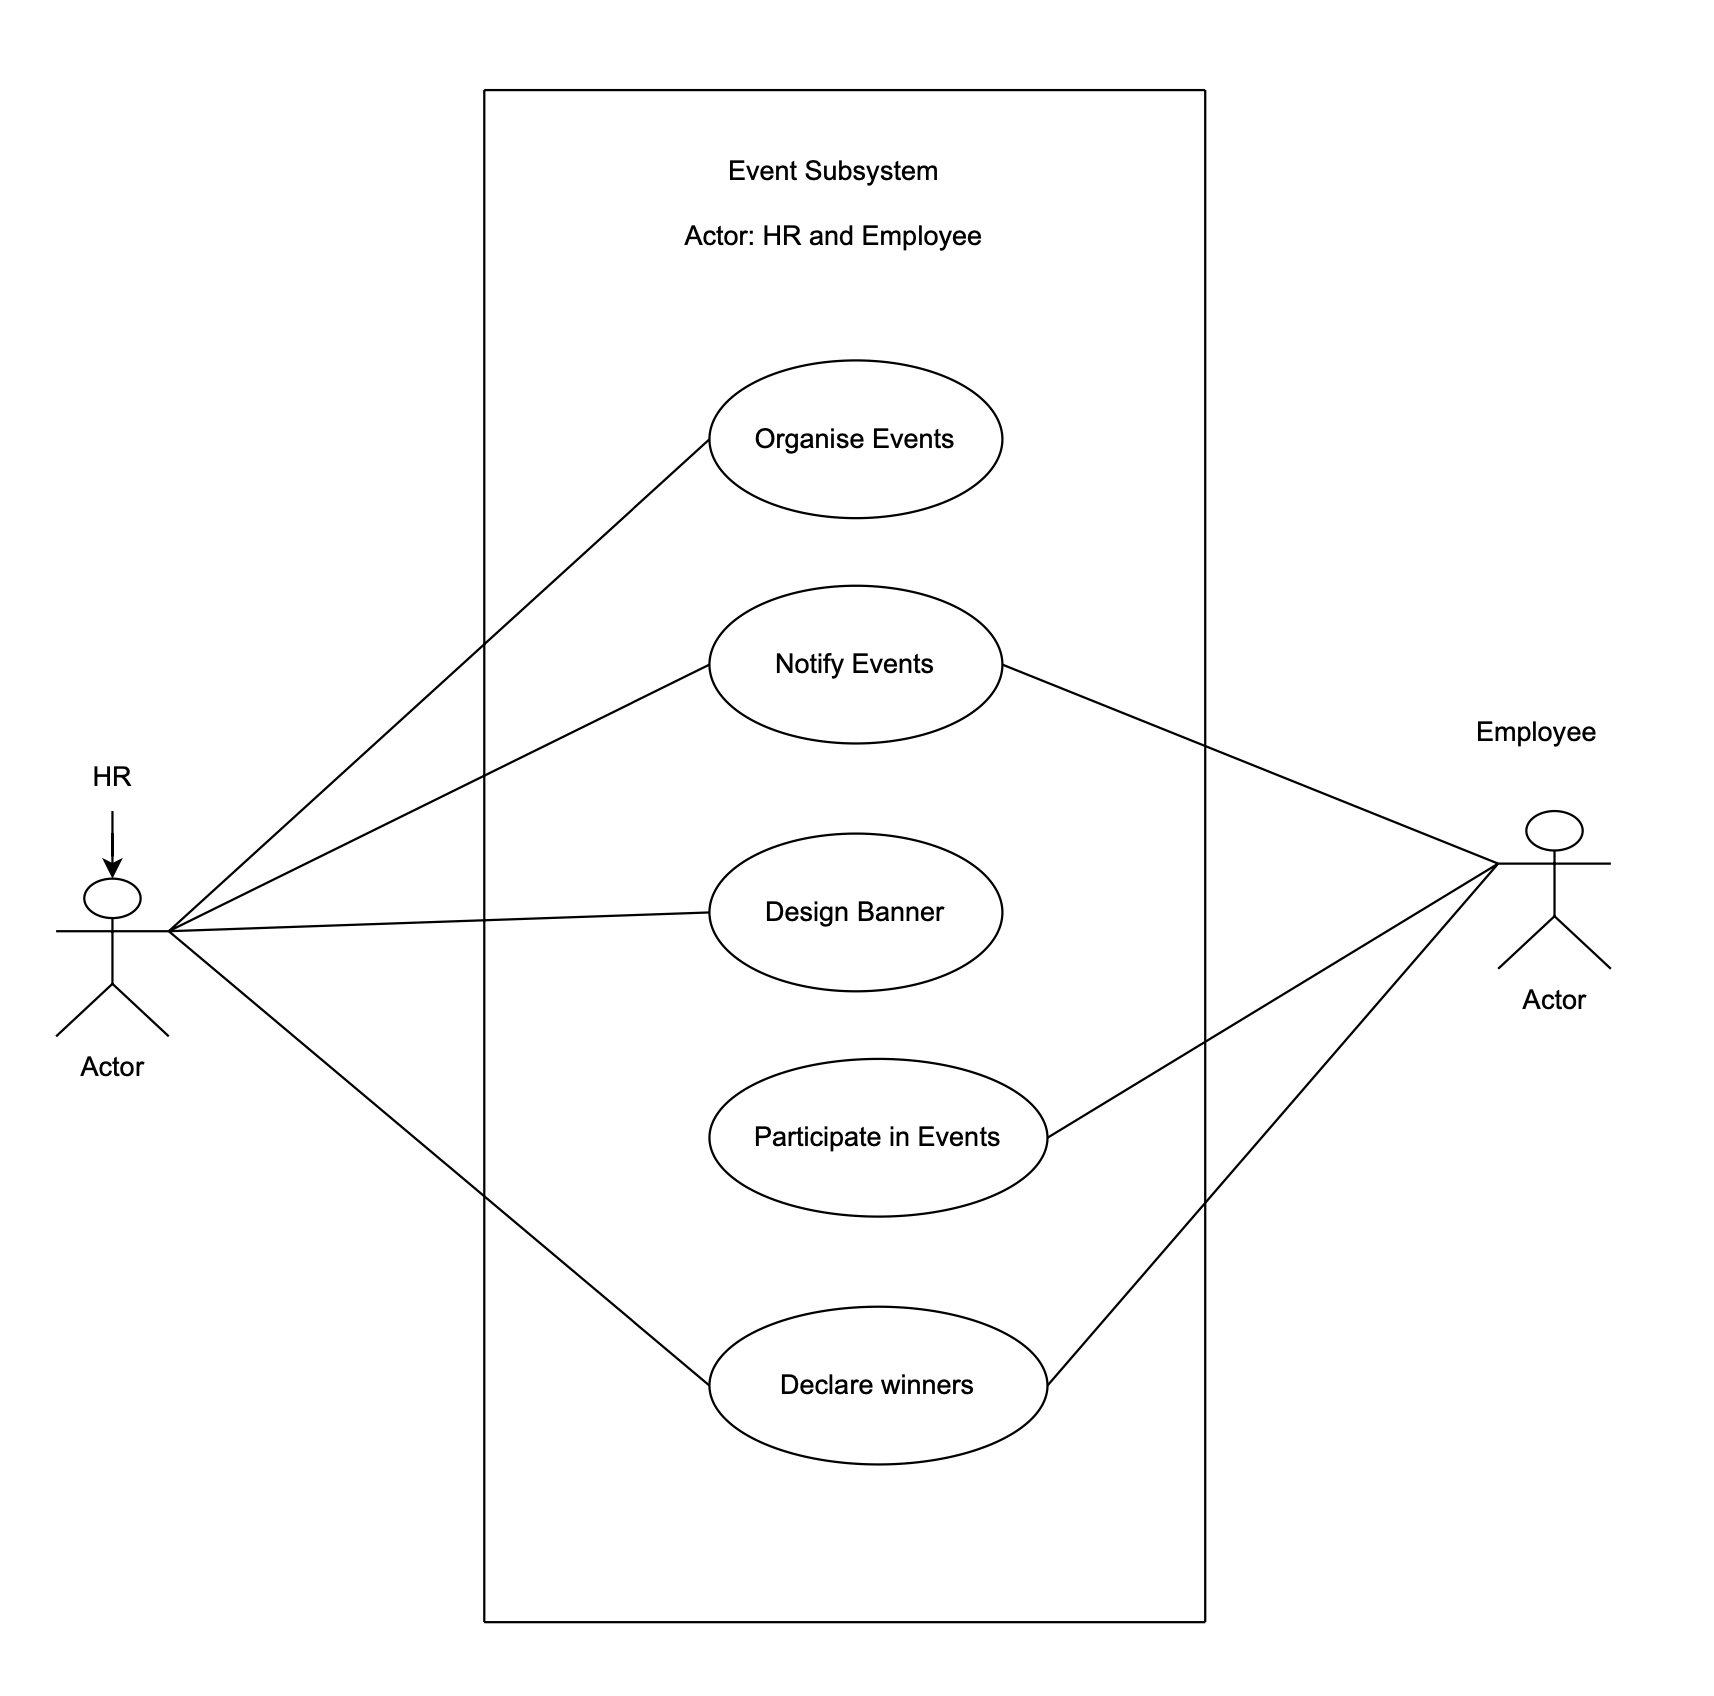
\includegraphics[width=\textwidth]
    {images/ucEvent.png}
    \caption{Use case diagram for Event subsystem}
    \label{fig:ucEvent}
\end{figure}

\begin{table}[h!t]
\caption{The Payroll Subsystem Use Cases}
{%
\newcommand{\mc}[2]{\multicolumn{#1}{#2}}
\begin{center}
\begin{tabular}{|c|c|}
\hline
\multicolumn{2}{|c|}{\textbf{RWIP Payroll Subsystem}} \\ \cline{1-2}
\textbf{Use Cases} & \textbf{Users/Actors} \\
\hline
\rule{0pt}{24pt} Get the list of winners in different Programs & Payroll Officer, Employee\\
\hline
\rule{0pt}{24pt}  Provide bonuses & Payroll Officer, Employee \\
\hline
\rule{0pt}{24pt}  Update Payroll & Payroll Officer \\
\hline
\end{tabular}
\end{center}
}%
\label{tab:payroll}
\end{table}

\begin{figure}[h!t]
    \centering
    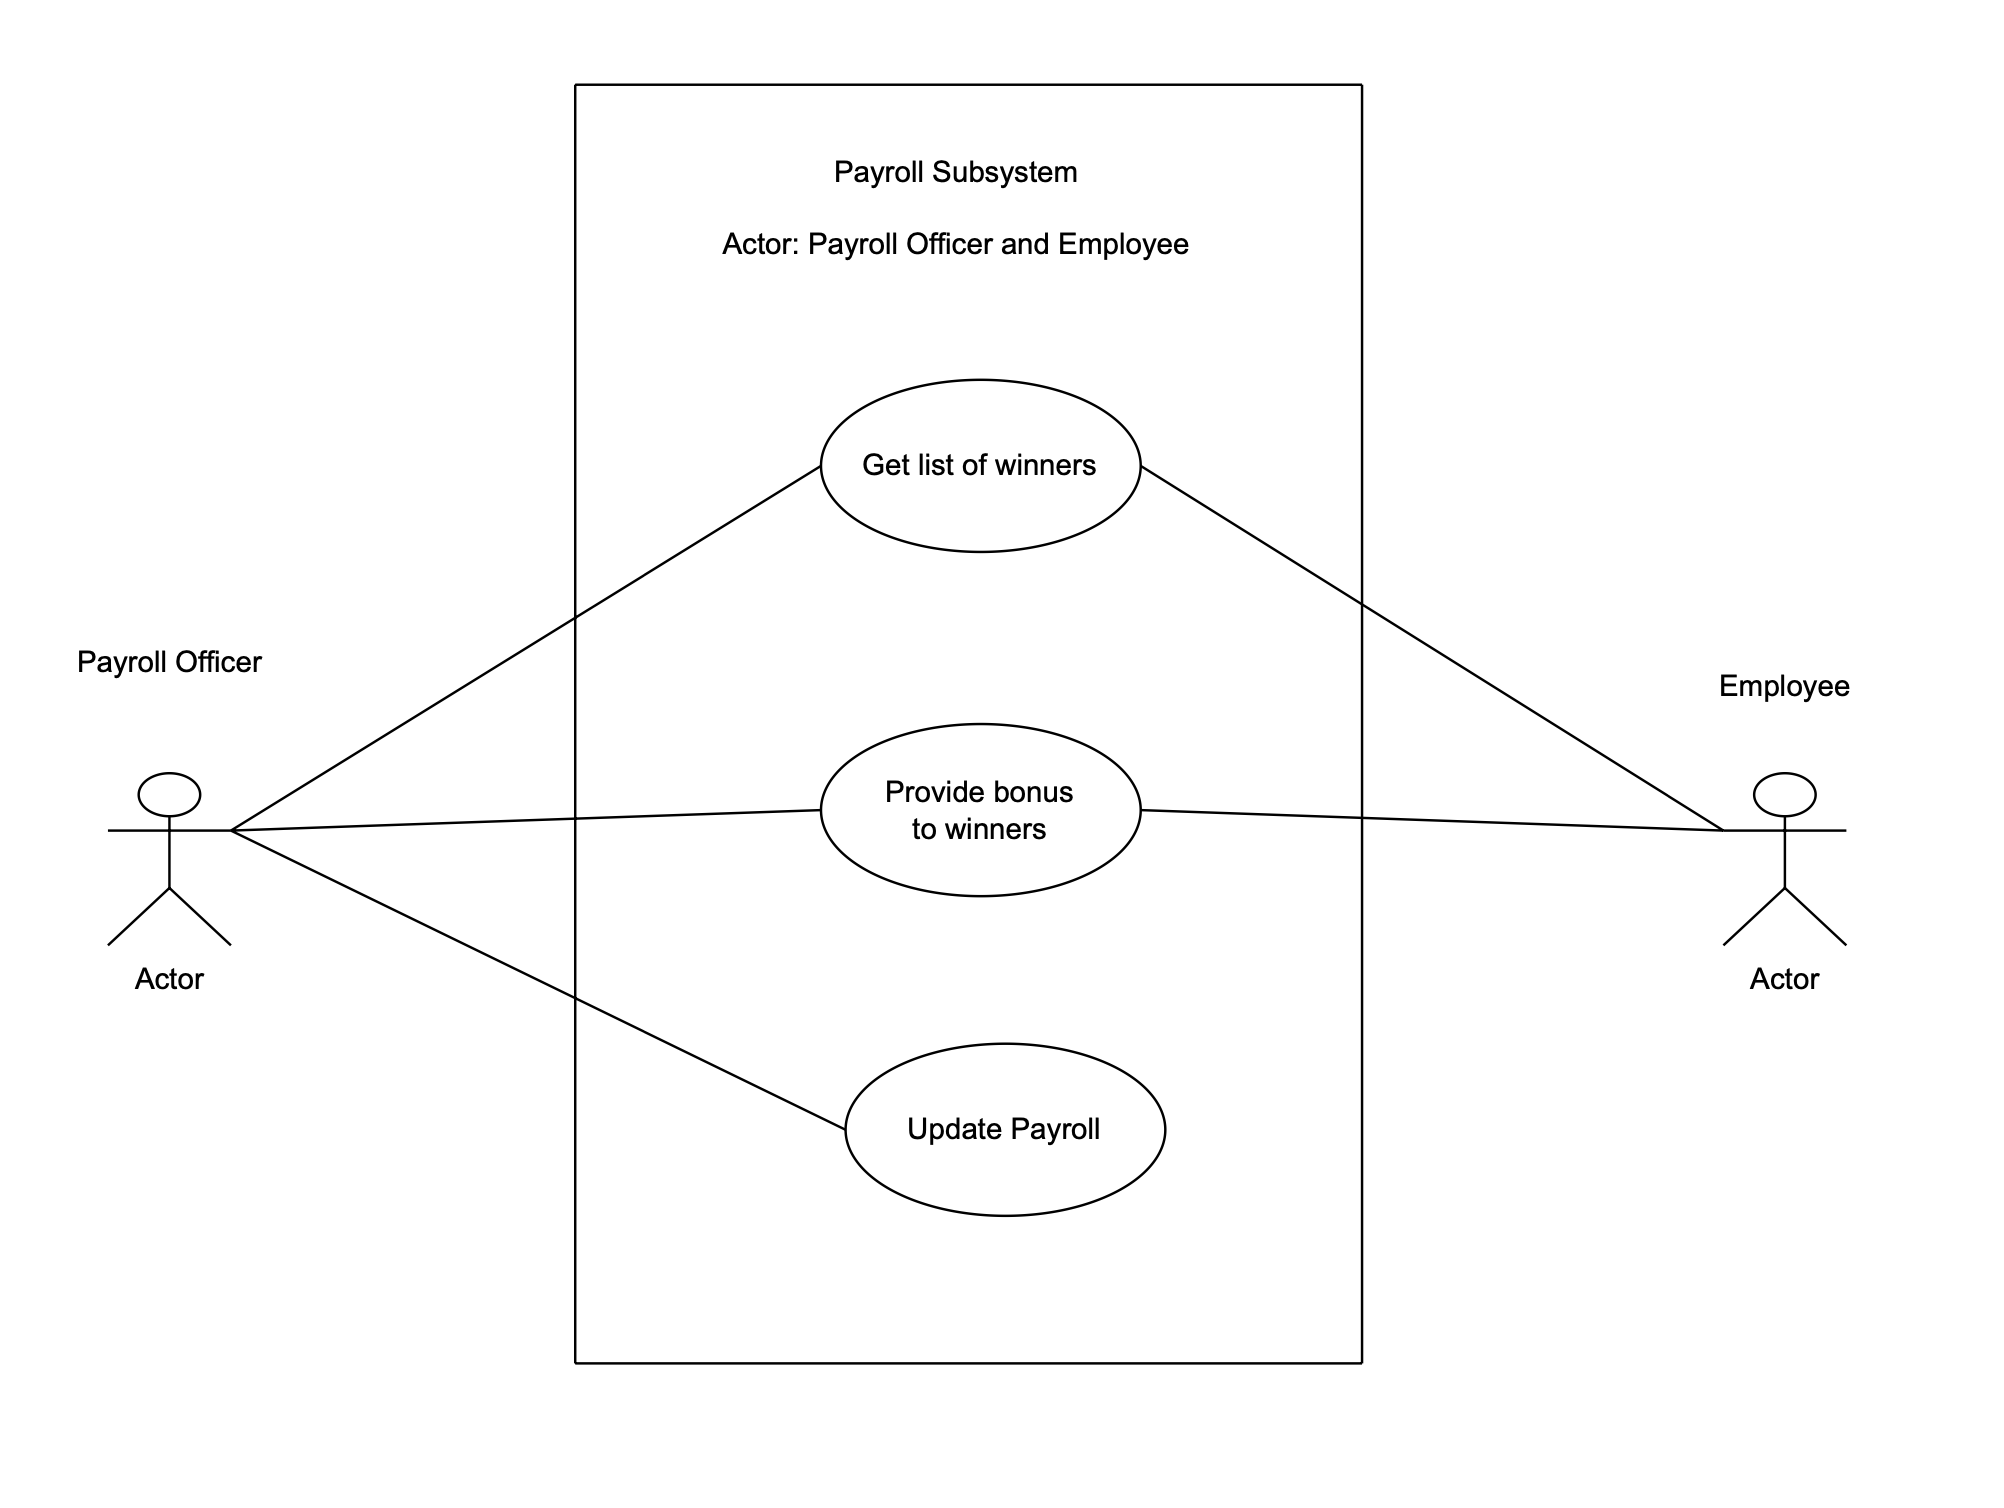
\includegraphics[width=\textwidth]{images/ucPayroll.png}
    \caption{Use case diagram for Payroll subsystem}
    \label{fig:ucPayroll}
\end{figure}

\begin{table}[h!t]
\caption{The Analysis Subsystem Use Cases}
{%
\newcommand{\mc}[2]{\multicolumn{#1}{#2}}
\begin{center}
\begin{tabular}{|c|c|}
\hline
\multicolumn{2}{|c|}{\textbf{RWIP Analysis Subsystem}} \\ \cline{1-2}
\textbf{Use Cases} & \textbf{Users/Actors} \\
\hline
\rule{0pt}{24pt}  Register as Admin & Analyst \\
\hline
\rule{0pt}{24pt}  Login as Admin & Analyst \\
\hline
\rule{0pt}{24pt}  Fetch Data & Analyst \\
\hline
\rule{0pt}{24pt}  Analyze Data & Analyst \\
\hline
\rule{0pt}{24pt}  Generate Report & Analyst, Developers \\
\hline
\rule{0pt}{24pt}  Make Decisions & Analyst \\
\hline
\end{tabular}
\end{center}
}%
\label{tab:analysis}
\end{table}

\begin{figure}[h!t]
    \centering
    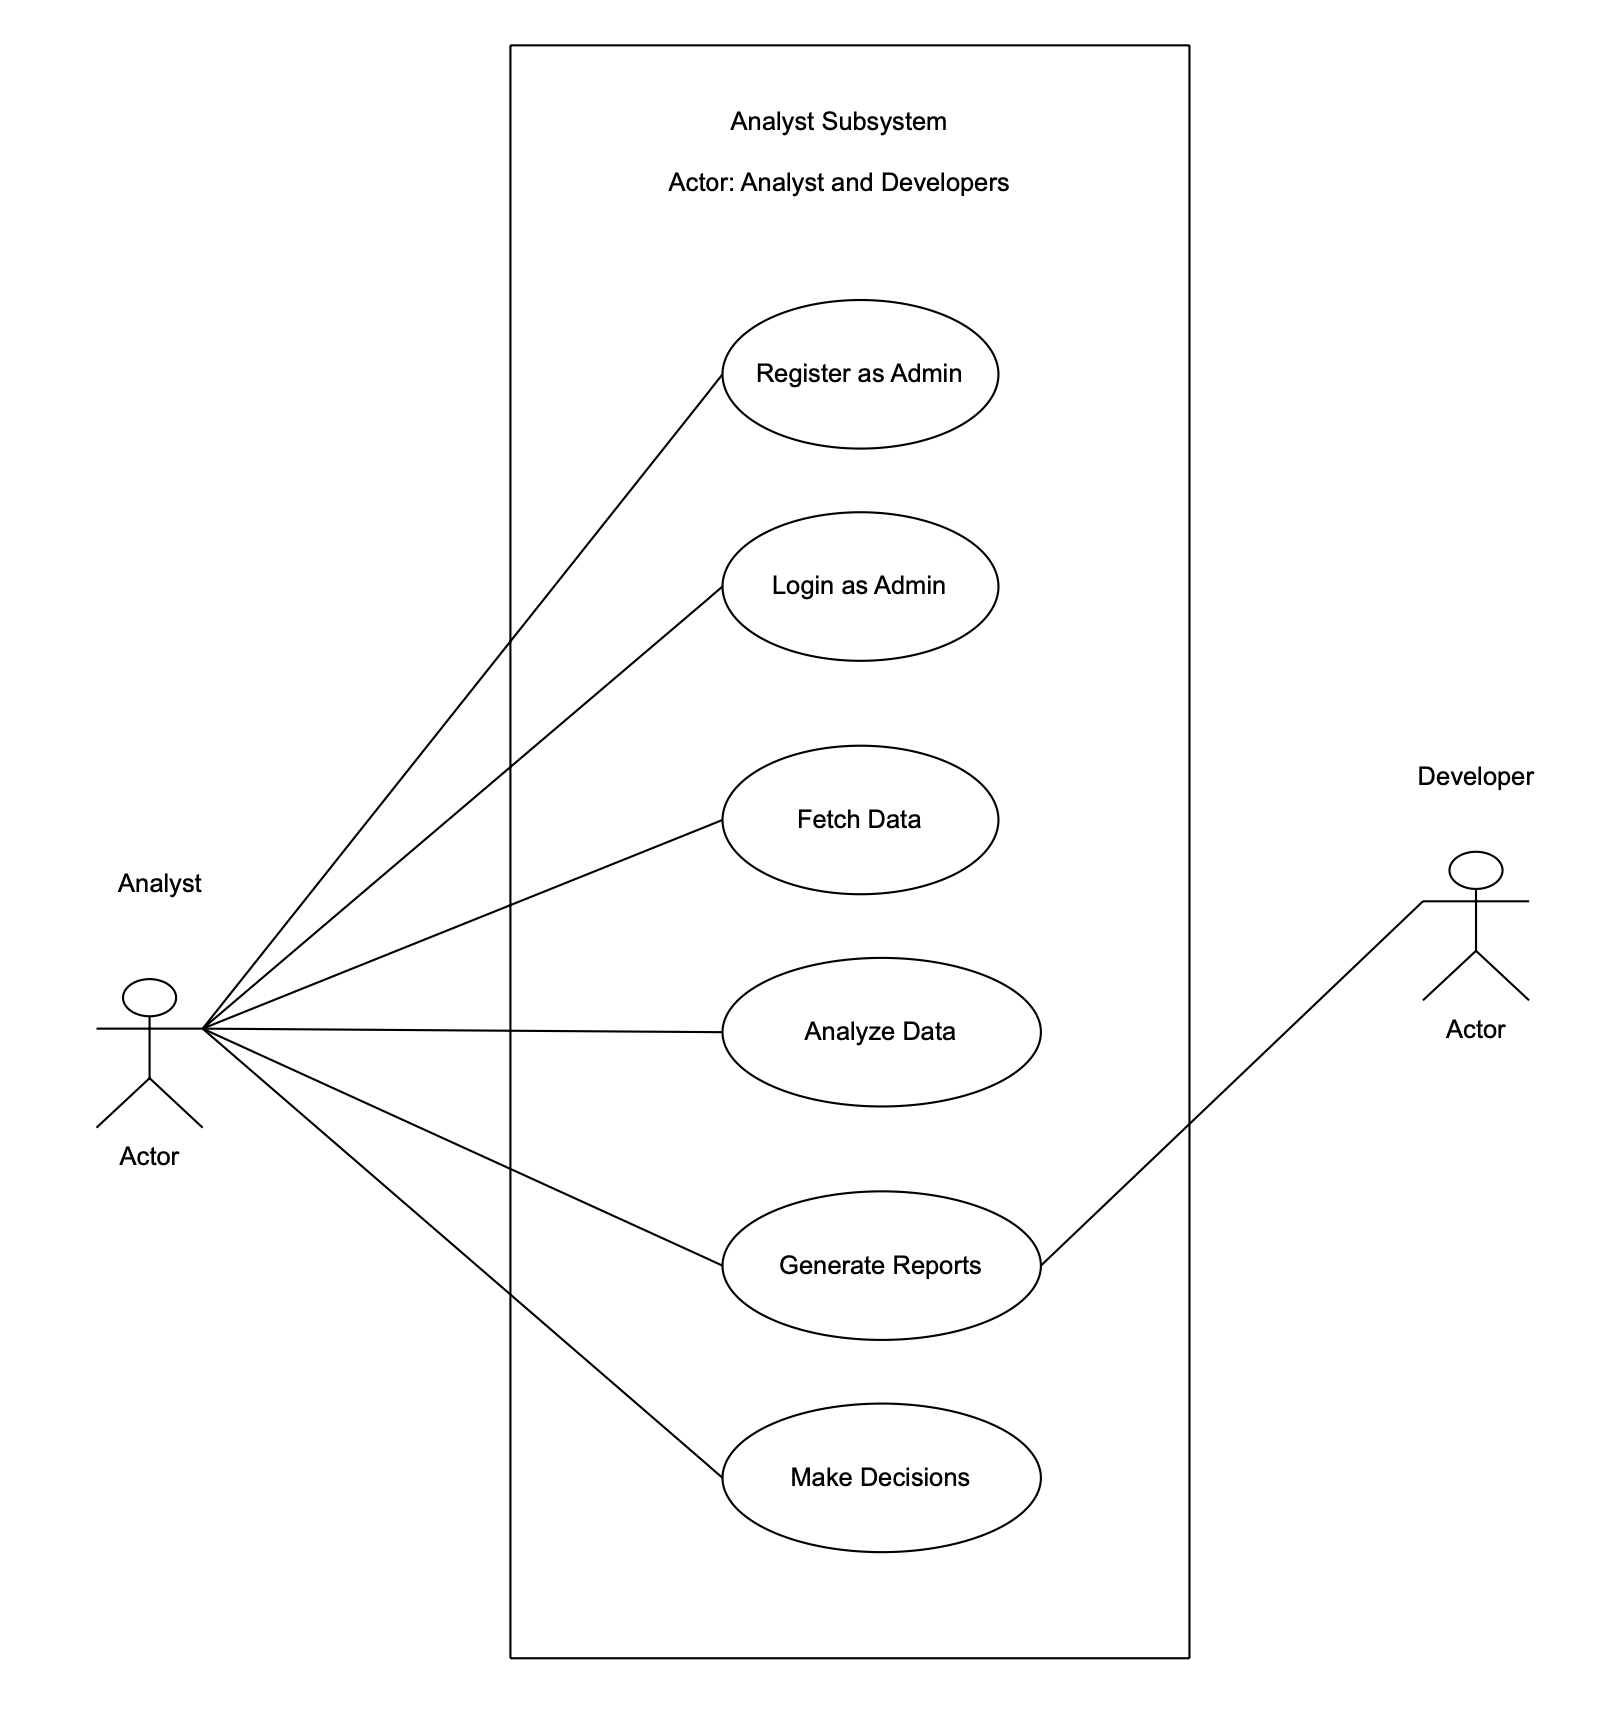
\includegraphics[width=\textwidth]{images/ucAnaysis.png}
    \caption{Use case diagram for Analysis subsystem}
    \label{fig:ucAnaysis}
\end{figure}


\section{Fully Developed Use Case Description}

\begin{table}[h!t]
\caption{Register/Create Account}

\begin{center}
\begin{tabular}{|c|c|}
\hline

\rule{0pt}{24pt}  \textbf{Use case name:} & Create employee account \\
\hline
\rule{0pt}{24pt}  \textbf{Scenario:} & Create online employee account \\
\hline
\rule{0pt}{24pt}  \textbf{Triggering event:} & Employee wants to join the recreational and wellness programs \\
\hline
\rule{0pt}{24pt}  \textbf{Brief description:} & Employee signs up or creates new account by providing their employee email id to access, book and participate in activity \\
\hline
\rule{0pt}{24pt}  \textbf{Actors:} & Employees \\
\hline
\rule{0pt}{24pt}  \textbf{Related use cases:} & Admin can create account on behalf of employee \\
\hline
\rule{0pt}{24pt}  \textbf{Stakeholders:} & Admin, HR \\
\hline
\rule{0pt}{24pt}  \textbf{Pre-conditions:} & Registration subsystem must be available \\
% Employees must have employer's provided email_id \\
% Employees must verify the account by clicking on verify link sent on the email
\hline
\rule{0pt}{24pt}  \textbf{Post-conditions:} & Employee account must be created and saved \\
% All the activity must be tracked like badge, rewards received.
\hline
\rule{0pt}{24pt}  \textbf{Exception conditions:} & Employee might not have email id provided by employer \\
% Employee have not verified the account by clicking on verification link sent on the mail.
% Email_id provided is invalid
\hline
\end{tabular}
\end{center}
\label{tab:createAccount}
\end{table}


\section{Sequence Diagram}

\begin{figure}[h!t]
    \centering
    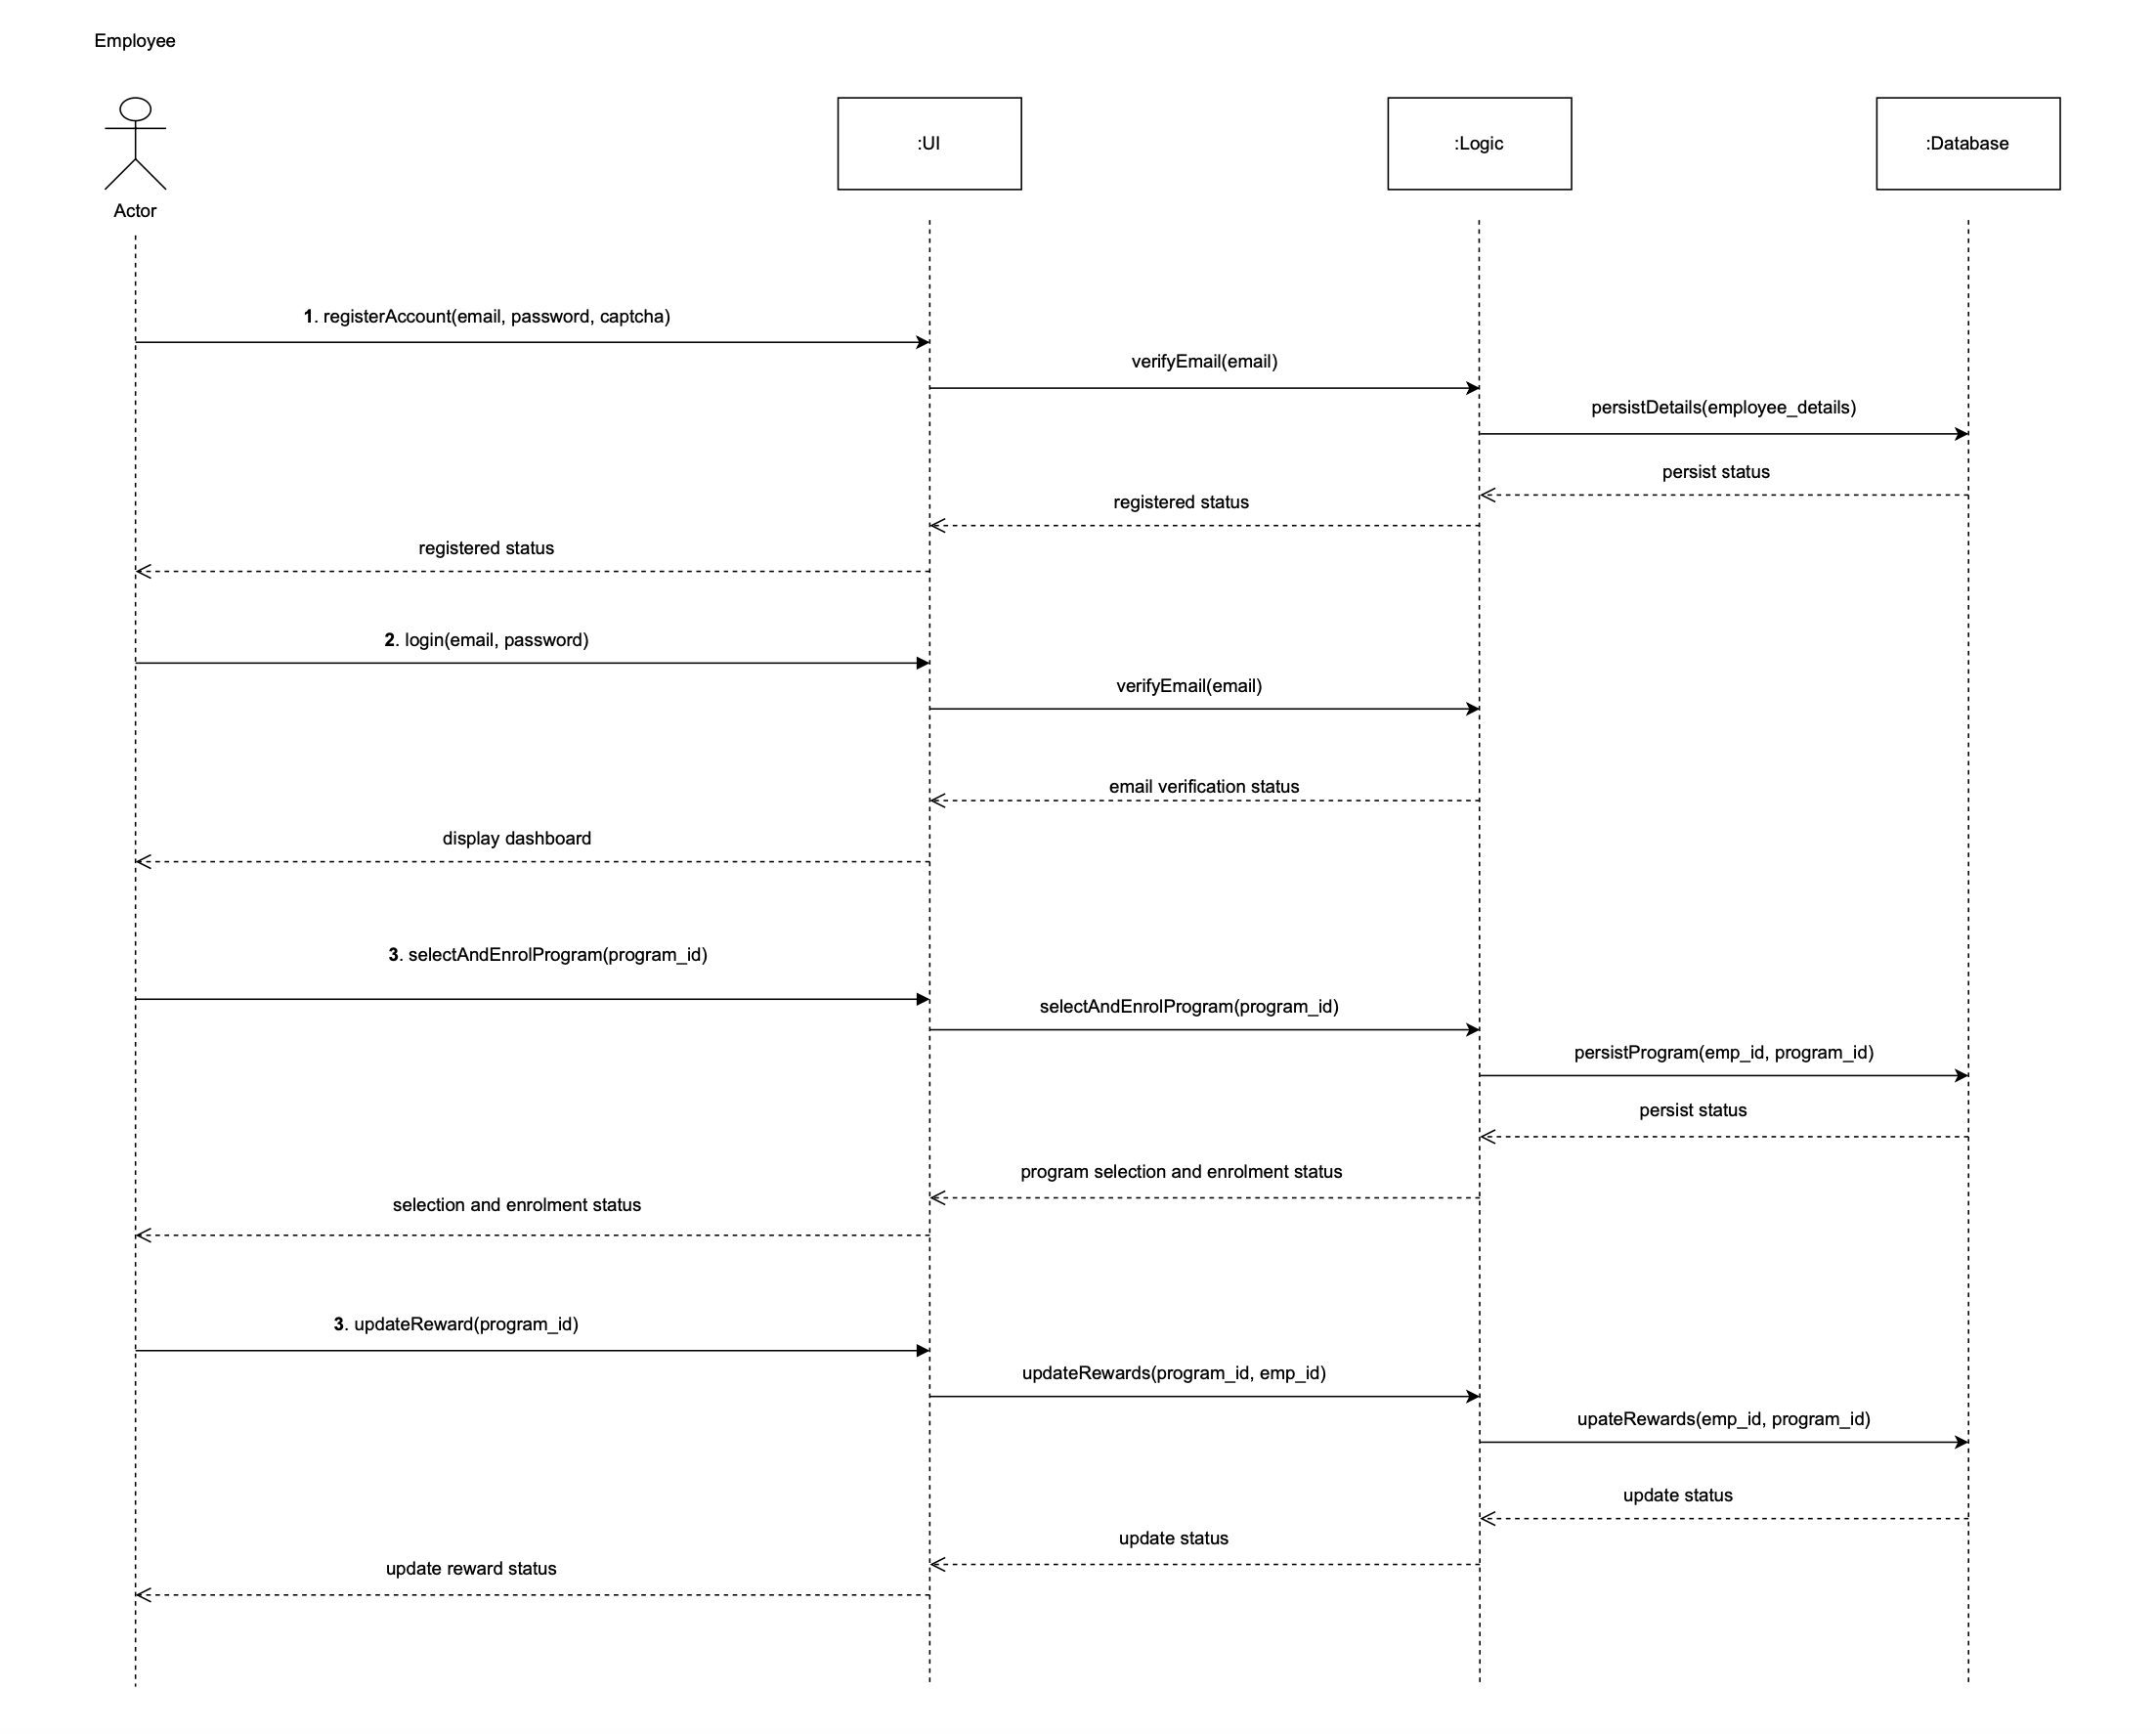
\includegraphics[width=\textwidth]{images/sequenceDiagram.png}
    \caption{Activity Diagram of all the subsystem}
    \label{fig:sequenceDiagram}
\end{figure}


\section{Activity Diagram}

\begin{figure}[h!t]
    \centering
    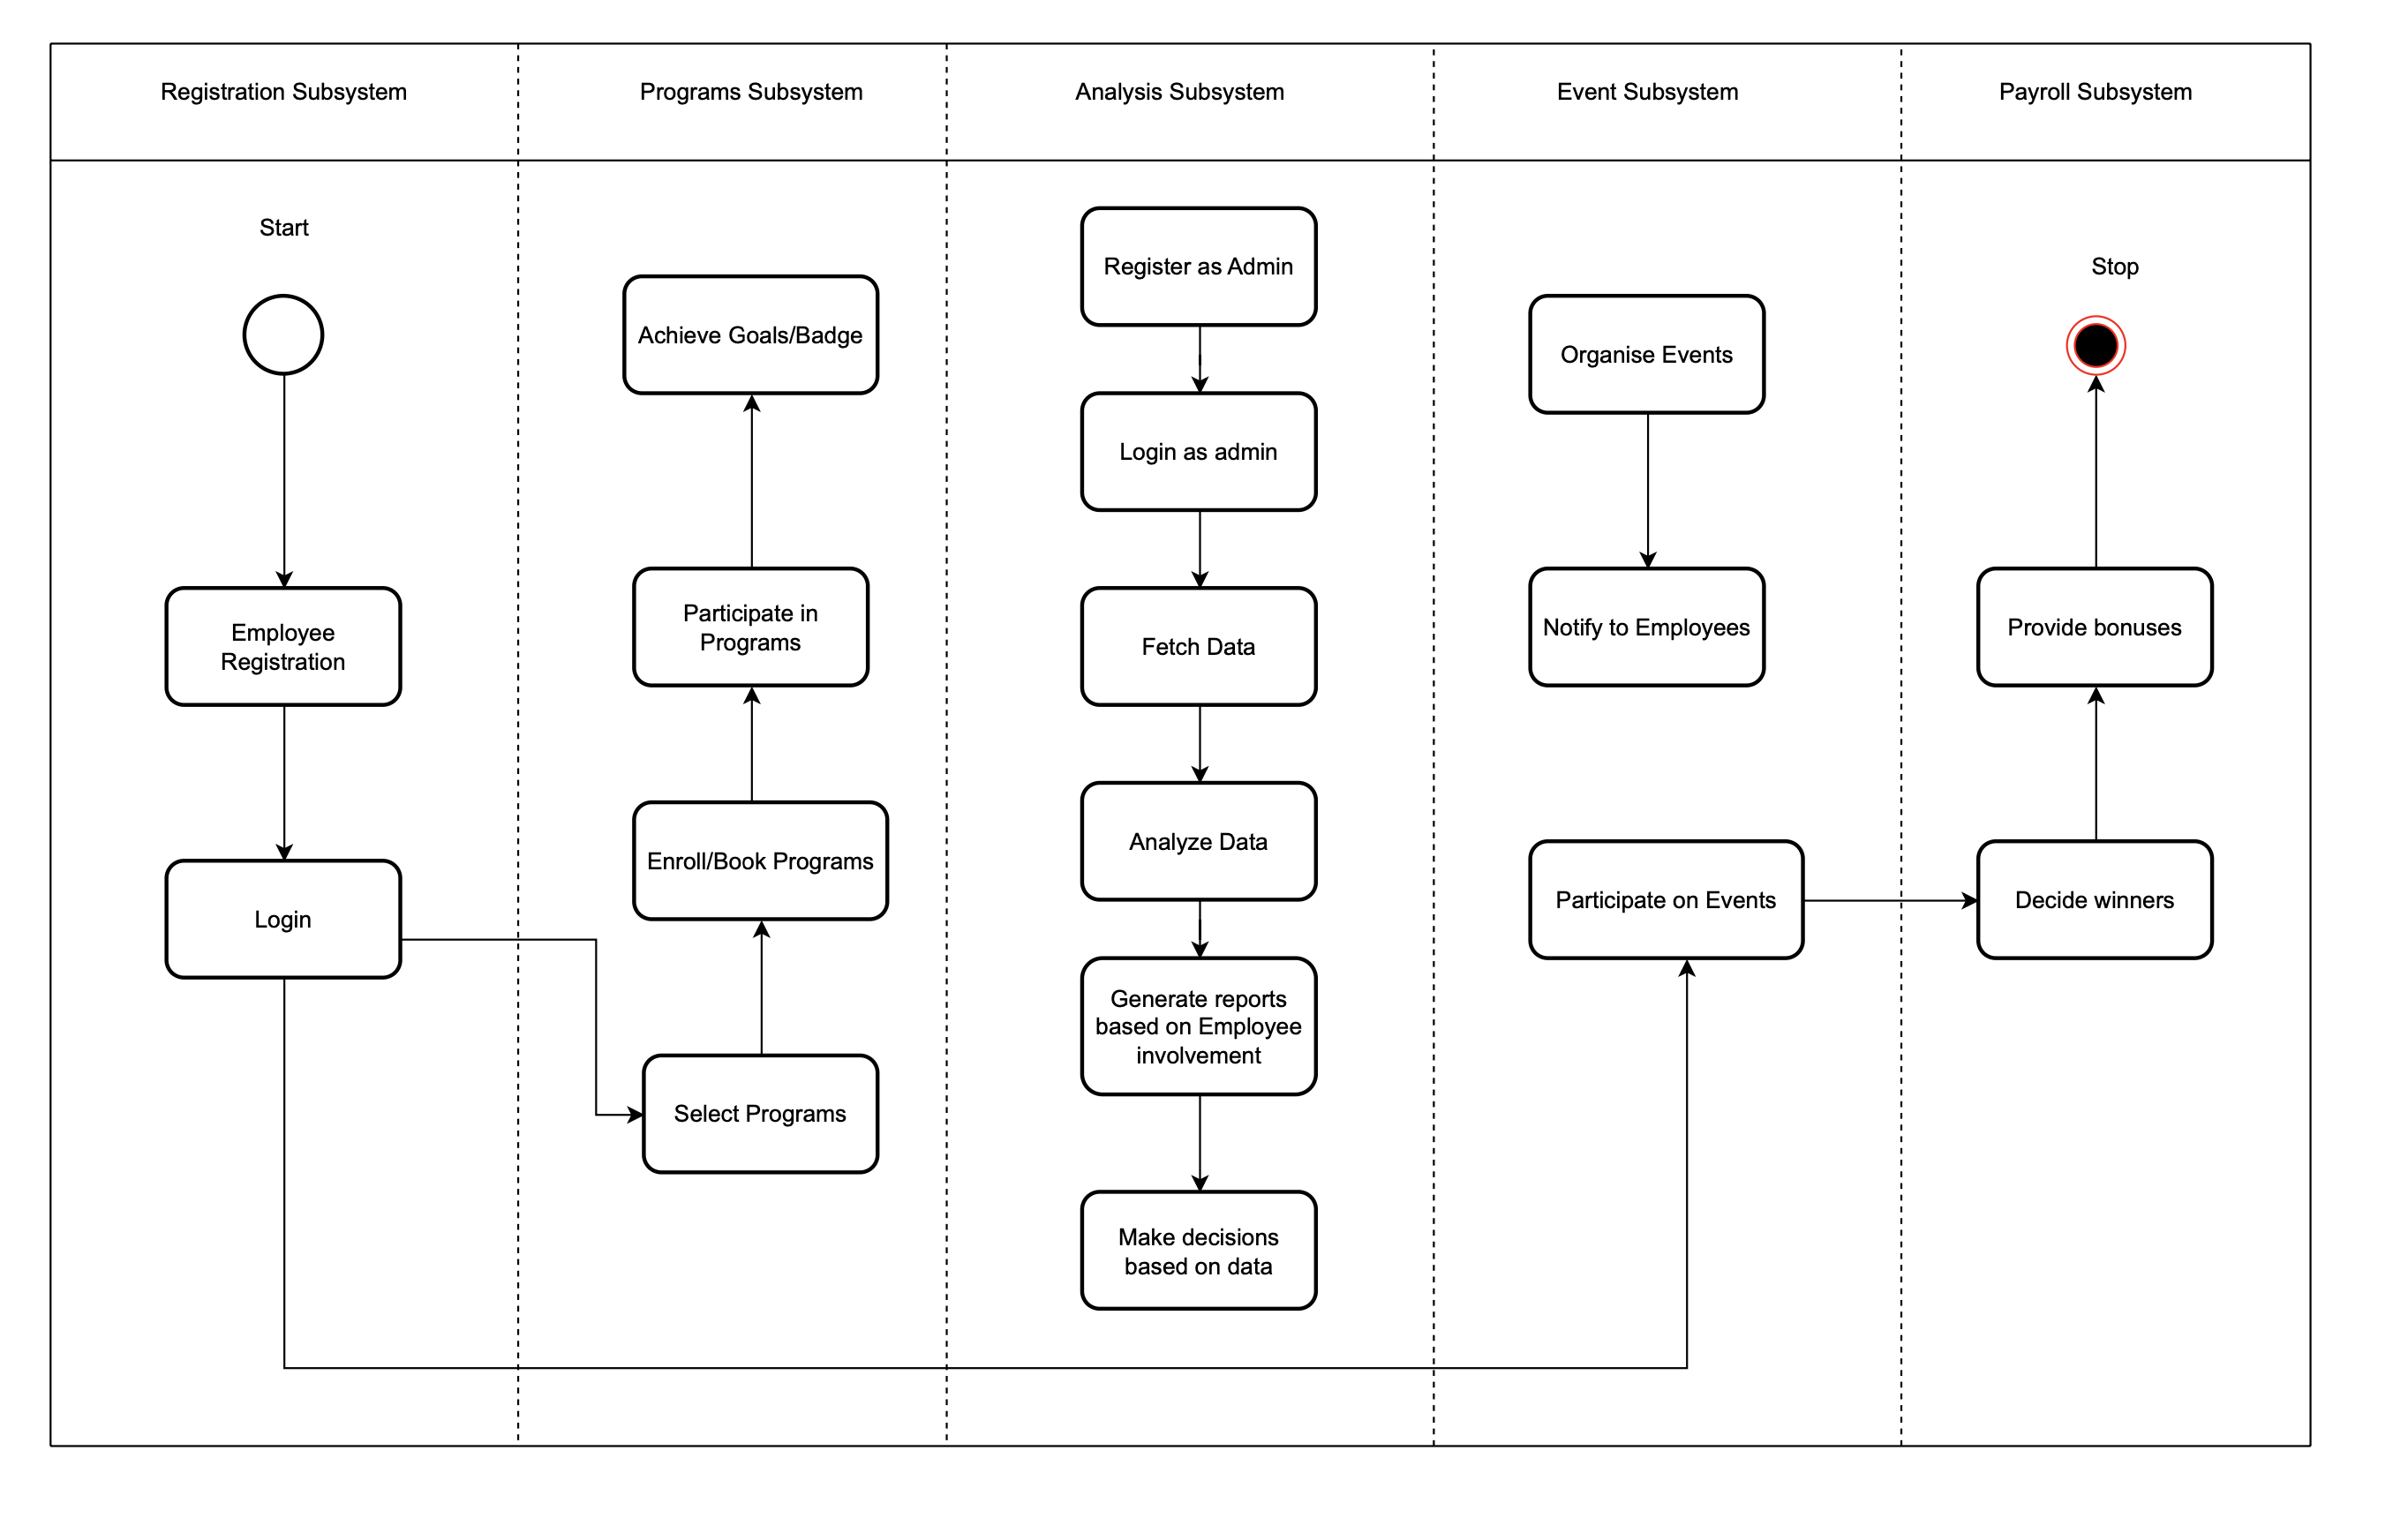
\includegraphics[width=\textwidth]{images/activityDiagram.png}
    \caption{Activity Diagram of all the subsystem}
    \label{fig:activityDiagram}
\end{figure}

\begin{figure}[h!t]
    \centering
    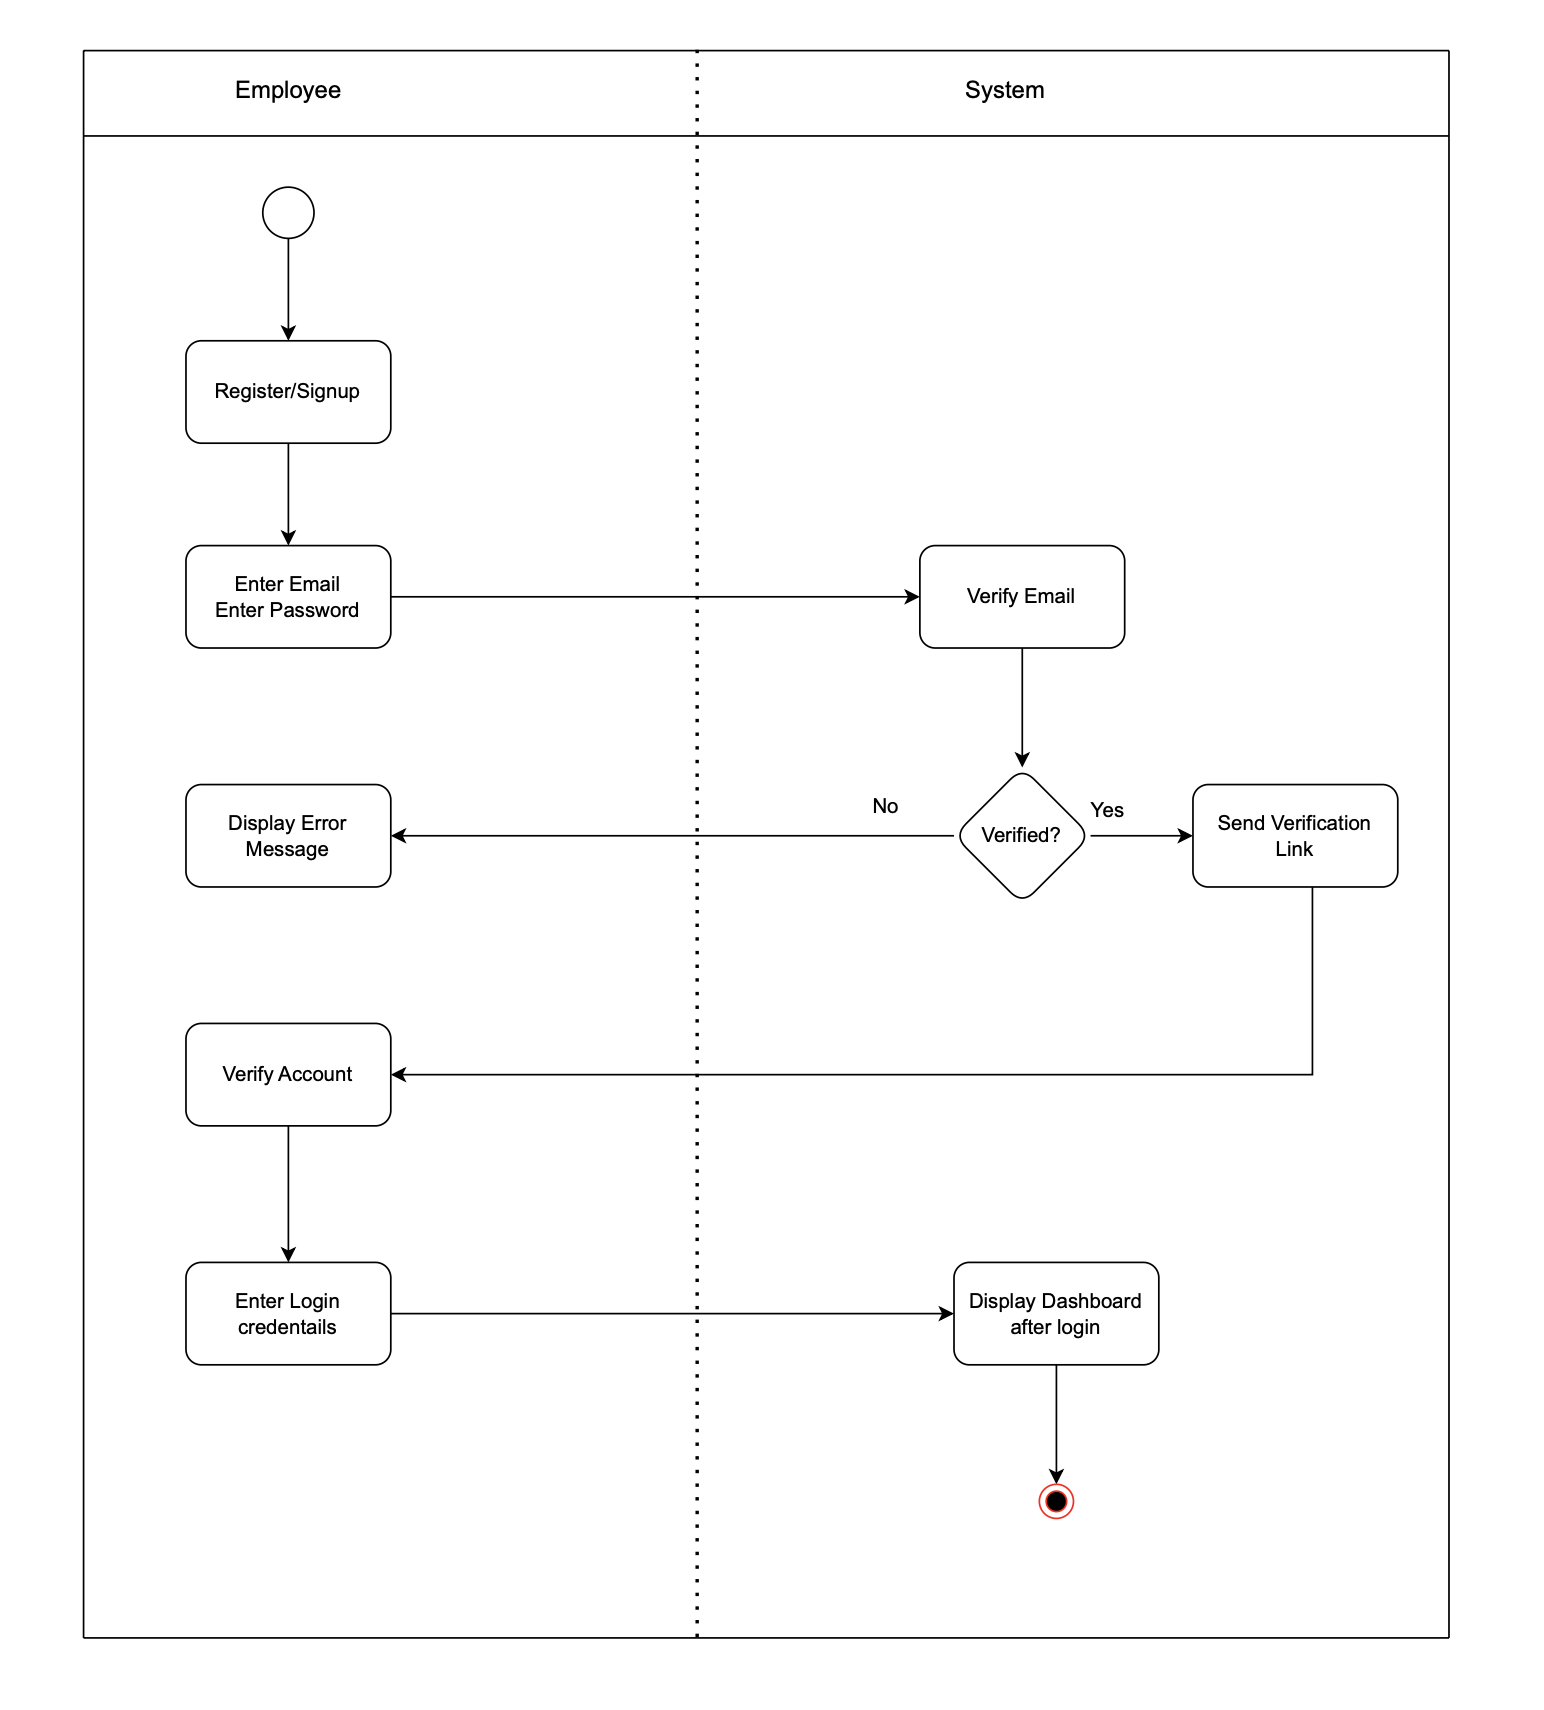
\includegraphics[width=\textwidth]{images/activityCreateAccount.png}
    \caption{Activity Diagram of Create Account use case}
    \label{fig:activityCreateAccount}
\end{figure}

\FloatBarrier
\newpage